\chapter{Experiments}

During the work on this thesis, various experiments have been conducted to find the correct parameters to use in subsequent development.
The following section provides details on the experiments done during this thesis to explain how the final results in the thesis have been achieved.


%Section 0: Hardware and software used in the project
%Hardware: Specify CPU/GPU/RAM etc used, available total storage (for flex?)

\section{Tools used in the thesis}
The following section lists the hardware and software used during the experiments in this master thesis.
It also lists tool-specific findings that are not relevant to mention in the other sections.

\subsection{Hardware}
\label{chex:hardware}

A table with the primary hardware used in this thesis can be found in \cref{tab:hardware}.

\begin{table}[ht]
    \centering
    \begin{tabular}{|c|c|c|c|c|}
        \hline
        Part type & Name & Main speed & Total memory size\\ \hline
        GPU & RTX 2080 Ti & 1.65 Ghz & 11 GB GDDR5\\ \hline
        CPU & Intel i7 4790k & 4.00 GHz & 32 GB DDR3\\ \hline
        Motherboard & Z97X-UD5H-BK & & \\ \hline
        SSD & 2x Samsung 860 EVO & 540 MB/s & 2TB \\ \hline
        HDD & 5x 12TB + 1x 10 TB & 160 MB/s & 70 TB \\ \hline
        Off. HDD & 5x 4 TB & 100 MB/s & 20 TB \\ \hline
        
    \end{tabular}
    \caption{Hardware specs}
    \label{tab:hardware}
\end{table}

In addition to the primary hardware, in several steps, processing was accelerated using other available PCs.
While helpful, the presented hardware has proven itself to be much faster than this alternative hardware, as noted in experiment 1 (data processing) and experiment x (iterative train root node). %Paranthesis and experiment numbers and text to be replaced by actual cref when these sections are done

The primary workhorse of the thesis is the GPU, the RTX 2080 Ti\cite{rtx2080}.
When the GPU is under minor load, the default clock is lower than advertised, at 1350 MHz.
The lower clock is due to the adaptive overclock features of the GPU.
Since the neural network processing does not utilize all GPU functions, and smaller models do not use the GPU to their fullest, the operating system lowers the clock speed to reduce heat.
To circumvent this and use the hardware to its fullest extent, one can start multiple Python consoles and train multiple neural networks in parallel.
In the case of the RTX 2080 Ti, up to 5 simultaneous threads have been used stably, with some limitations.
During full utilization of the GPU, clock speeds above 1920 MHz have been recorded, while maintaining temperatures below 60 degrees celsius.
As at that point, resource utilization is at its fullest; network training time is increased for each individual thread. 
However, the total processing time is still reduced as hardware is utilized more overall.

One problem that has arisen during development was the lacking capabilities of other hardware when compared to the GPU.
The RTX 2080 Ti was purchased in late 2019 for the thesis, while the CPU and RAM were purchased in early 2015.
Running multiple Python consoles includes having the cache for each console in RAM.
Python is not a memory-optimized scripting language, and uses much space for each variable in memory\cite{theano:memory}.
While the amount of RAM available on the hardware is above the standard of desktops built even today, maxing the capacity of the motherboard, some experiments have still been limited in running more simultaneous processes due to RAM shortage.
Also, the limitation of the quad-core nature of the CPU has been a limiting factor in the more CPU intensive tasks in the thesis, most notably experiment 1.%cref
Tasks that only run on the CPU like data preparation and even python consoles themselves during neural network processing need a minimum amount of CPU resources to function properly.
Even if the RAM issue was resolved, the limited number of CPUs would block more than 5 python consoles running simultaneously.

In terms of findings on storage and caching, when using Pythons pickle library, storing the dataset on an SSD will improve read times by an estimated 35\% over using HDDs.
According to a speed test done on the hardware, the read-time of an SSD is around 540 MB/s, while the read-time of the tested HDD is around 160 MB/s.
Therefore, the benefits of moving the dataset to a faster medium is entirely dependent on the size of the dataset, and frequency of changes to the dataset.
In the case of this thesis, experiment x (root node) used the SSD as a cache for the dataset.%cref
In contrast, experiment y (trees) used almost all available HDDs for the dataset cache, excluding the external drive.%cref
Given the nature of the last experiment, each experiment variation would need a full copy of the dataset.
Also, these copies of the dataset would be repeatedly created and deleted, adding to the wear of the drive.
Each experiment variation was given a dedicated drive to alleviate the potential performance loss due to drive seeking present on HDDs, with the results also being printed to a dedicated drive.
As mentioned, the external drive was not used as a dedicated drive, due to lower performance compared to the internal drives operating over SATA-3.

It is also important to mention the massive data storage pool of the hardware.
Thanks to the available storage, each step of the dataset generation could be stored for safe-keeping.
Large amounts of free storage also enabled various storage-expensive methods of caching, as mentioned above.
Also, multiple older HDDs have been used as backups and portable storage for the dataset.

\subsection{Software}
%Software: Specify Python + Tensorflow versions (2.0 early on, 2.1 later, 2.2 available in the end but not used)
%Software python: Include info on Librosa, Scikit and other large libraries used and why
The development platform used during this thesis has primarily been Python on a Windows 7 computer.
\cref{tab:software} details the different versions of the software used for development in the thesis.

\begin{table}[ht]
    \centering
    \begin{tabular}{|c|c|c|c|c|}
        \hline
        Name & Version\\ \hline
        Anaconda & 2019.10\\ \hline
        Python & 3.7\\ \hline
        TensorFlow & 2.0, 2.1\\ \hline
        TensorBoard & 2.0, 2.1\\ \hline
        Librosa & 0.7.2\\ \hline
        Scikit-learn & 0.22.2\\ \hline
        Spyder & 3.3.6, 4.1.2\\ \hline
        PowerShell & 5.1\\ \hline
        FFmpeg & 4.2\\ \hline
        
    \end{tabular}
    \caption{Software versions}
    \label{tab:software}
\end{table}

\subsubsection{Python environment}
%Python 3.7
A Python environment requires a package manager to use it to the fullest extent.
Visual Studio that the student has already had installed on the computer also included a full Python environment with Anaconda\footnote{\url{https://www.anaconda.com/}}.
While the included version has proven itself to be unreliable and required multiple re-installations, certain features have proven themselves to be necessary throughout this thesis.
The most crucial feature that prioritized Anaconda over picking pip was the ability to create separate virtual environments with different versions of packages installed simultaneously.
Individual packages often require specific versions of dependencies that may not be available anymore, in which case an outdated version of the package may be installed without notice to the user.

%Librosa for dataset, mention trouble with version in Anaconda
One case of the separate environments being critical for this thesis was the Librosa\footnote{\url{https://librosa.github.io/librosa/index.html}} library.
Librosa is a python package for music and audio analysis, which this thesis used to process the dataset with the various feature extraction methods that Librosa supports.
Deep in the dependency chain for Librosa, a dependency conflict arose that forced Anaconda to install version 0.6.3 of Librosa, while the latest current version is 0.7.2.
As the feature extraction methods are based on scientific algorithms and thus should not change between versions, each new version of a package can include more methods that the user expects to have available.
A separate environment dedicated exclusively for Librosa had to be developed to handle this dependency conflict to resolve the matter in the thesis.


%Tensorflow 2.0, 2.1 later on
The Tensorflow\footnote{\url{https://www.tensorflow.org/}} package was selected for the development of the thesis to create and train neural networks.
As Google develops TensorFlow, one of the leading firms in Artificial Intelligence research that also employs researchers that published the Inception paper\cite{szegedy2014going}, it was picked as the superior choice.
Shortly before the thesis project started the development of neural networks, version 2.0 of Tensorflow was released.
This thesis used version 2.0 at the beginning of the thesis, updating to version 2.1 in the middle of the thesis.
Version 2.2 was released in the final month of the thesis. 
While certain features that were released in this version would be exciting to use during development, it was not used to maintain the stability of the thesis results.

As noted in the hardware section, multiple Python consoles have been used to train multiple neural networks simultaneously.
To achieve this, Tensorflow needs to be configured only to use a limited amount of memory on the GPU.
Under regular operation, Tensorflow will attempt to use all available memory for itself, which will lead to potential system instability and hanging even if only one network is trained at a time.
Because of the recent update from 1.x versions of Tensorflow, a compatibility layer needs to be used in current versions of Tensorflow as the equivalent functionality has not been found in versions 2.0 and higher.
The memory fraction parameter has to be changed to the desired level to adjust the maximum memory used by Tensorflow, code for which is provided in the code listing below.
It is important to note that the memory fraction does not represent the actual memory fraction used by Python, and is a significant percentage higher than the parameter set in the code.
A tool provided by Nvidia called Nvidia SMI had been used to monitor resource utilization during the development of the minimal parameters that could provide a stable and fast environment.

\lstinputlisting[
    caption={Code to reduce memory usage of Tensorflow in a single console, valid for Tensorflow 2.1},
    label=lst:pythonfile,
    language=Python
]{listings/memcode.py}

%Tensorboard for experiment results
The Tensorboard\footnote{\url{https://www.tensorflow.org/tensorboard}} package was used to process the results of the various experiments detailed in the later sections of this chapter.
Tensorboard is a visualization toolkit developed for Tensorflow.
The primary feature used in the toolkit was the ability to record, view, and sort individual neural network tests.
As Tensorboard integrates easily in Tensorflow, this allowed for agile development of the test code, where tests were rapidly coded, run, and analyzed.
However, given the sheer amount of tests run during this thesis, the thesis has stumbled across a critical performance bug.
Tensorboard attempts to record the state of the neural network as it is trained, and recreate a visual graph for the training process.
While this may be a useful feature for other projects, it was not relevant for this thesis, while simultaneously causing some experiments to max out the RAM on the computer.
The features that cause this bug to manifest can be disabled by using Anacondas' capacity to create custom environments, creating an environment exclusively for Tensorboard.
Other packages can also be installed in this environment; however, Tensorflow has to be explicitly excluded from this environment.
Doing so causes Tensorboard to enter a restricted feature mode, which allows for much larger tests to be viewed with minimal lag.

%Scikit-learn for clustering
%Spyder IDE, Anaconda environment
%Pickle for data saving
In addition to the above packages, several other packages have been used extensively in the project.
To create the hierarchical clusters for the first clusters, scikit-learn\footnote{\url{https://scikit-learn.org/stable/index.html}} has been used.
Scikit-learn provides a lot of various functions that are useful in neural network development.
For the IDE, Anaconda comes pre-installed with Spyder\footnote{\url{https://www.spyder-ide.org/}}, which was used for the development of the thesis.
Lastly, the pickle package in Python was used to save results to disk, along with handling cache logic.


\subsubsection{Other}
%Powershell for dataset s1 and s2
%FFMpeg for dataset extraction, processing
In addition to using Python during most of the development, Powershell was used in the early stages of dataset preparation.
Powershell was chosen for these first tasks due to earlier experience in using Powershell to maintain the media library used as the dataset in the thesis.
As Powershell would be satisfactory in the first tasks, it was chosen to be used over Python due to students lacking experience in using Python at the time.
Since the data extraction script was intended to be run only once, writing the scripts quickly and starting to develop Python code was preferable, especially given the expected time to process the dataset.
The Powershell version used in the thesis was 5.1.

The media converter FFmpeg\footnote{\url{https://ffmpeg.org/}} was used to facilitate the processing of the dataset into a standardized form.
FFmpeg supports a wide variety of video, audio, and subtitle formats.
The ability to process any input was critical when various video files in the dataset had an unknown number of codecs used to encode them.
Some of the more recent media may use more modern formats, while older media may use some more obscure format that other tools could fail to process.
As each sample in the final dataset needed to carry only the particular subtitle fragment, the ability to specify file length options with a command line was also necessary for the selection of the conversion tool.
Since losing samples due to shortcomings in the selected tool would be undesirable, FFmpeg fit the requirements the most.
The FFmpeg version used in the thesis was 4.2.



%Section 1: Dataset selection, why mfcc dct 3 and others got picked, here is actual first nn development
\section{Dataset selection}
\label{ex:dataset}

The goal of this experiment was to investigate if neural networks could produce any relevant results for the thesis and determine which of the function combinations would be best suited to proceed with.
\subsection{Experiment setup}
The first experiment revolved around a minimalist neural network to select the appropriate function combination to use in Librosa to generate the dataset for the rest of the thesis.
A table detailing each layer in the network can be seen in \cref{tab:earlymodel}.

Three one-dimensional convolution layers start the network, followed with a standard max pool layer.
An operational flattening layer is added to make the layers fit into the dense layers.
One dense layer is added before the final two layers, to serve as an abstraction of the input data.
Then, a dense layer with the softmax activation function is added to the network.
The softmax layer serves as the classification layer, forcing the network to pick one of the neurons to classify the sample into.
An extra dense layer is added with the sigmoid activation function to represent the dataset
This layer represents the dataset used in this experiment, and each sample maps to their neuron in this layer.

\begin{table}[ht]
    \centering
    \begin{tabular}{|c|c|c|}
        \hline
        Layer type & Parameters & Activation\\ \hline
        Conv1d & 64 filters, size 3 & ReLU\\ \hline
        Conv1d & 64 filters, size 3 & ReLU\\ \hline
        Conv1d & 64 filters, size 3 & ReLU\\ \hline
        Max pool & Size 2 & ReLU\\ \hline
        Flatten & &\\ \hline
        Dense & 250 & ReLU\\ \hline
        Dense & 10 & Softmax \\ \hline
        Dense & 1000 & Sigmoid \\ \hline
    \end{tabular}
    \caption{Early neural network model}
    \label{tab:earlymodel}
\end{table}

The process of getting the results can be summarized as follows:
\begin{itemize}
    \item Train a fresh network on the entire dataset.
    \item Remove the last layer
    \item Run a prediction on the dataset
    \item Generate a new instance of the network, minus the last layer
    \item Train the network on the dataset using a 70\% train and 30\% validation split
\end{itemize}{}

By creating a new network and training the network based on the results of the first, the goal was to determine if the network was able to find any features to group samples autonomously.
To control for potential overfit errors, in addition to the standard validation loss and accuracy values, the number of classes and the size of the largest class was tracked.
Therefore, the best result would be the function combination that achieved the best performance in all three combinations.

\subsubsection{Dataset}
Using the entire dataset for this experiment was not yet possible, both because it did not exist in the correct form yet, and that the neural network was built to handle only one thousand networks, to begin with.
For this experiment, a selection of around 38 thousand samples were processed in all function combinations.

The function combinations could consist of the following options:

\begin{itemize}
    \item FFT window size: 1024, 2048, 4096
    \item n\_chroma: 12, 24, 48
    \item DCT: 2, 3
    \item Power: 1, 2, 3
    \item Order: 0, 1, 2
    \item Center: True, False
\end{itemize}{}

The functions that were considered and the parameters that were tried with them are presented in \cref{tab:ex1dataset}.
In total, 67 possible combinations were tried.

\begin{table}[ht]
    \centering
    \begin{tabular}{|c|c|}
        \hline
        Function type & Parameter type\\ \hline
        chroma\_stft & FFT, n\_chroma\\ \hline
        chroma\_cqt & n\_chroma\\ \hline
        chroma\_cens & n\_chroma\\ \hline
        melspectrogram & FFT, Power\\ \hline
        mfcc & DCT\\ \hline
        rms & FFT\\ \hline
        spectral\_centroid & FFT, Center\\ \hline
        spectral\_bandwidth & FFT\\ \hline
        spectral\_contrast & FFT, Center\\ \hline
        spectral\_flatness & FFT, Power\\ \hline
        spectral\_rolloff & FFT\\ \hline
        poly\_features & FFT, Order\\ \hline
        tonnetz & \\ \hline
        zero\_crossing\_rate & \\ \hline
    \end{tabular}
    \caption{Librosa functions that were tested}
    \label{tab:ex1dataset}
\end{table}

\subsubsection{Control group}

A control test was run to verify that the network achieved a useful result.
The control test consisted of training the neural network model on a randomly generated group of classes.
Should the experiment be successful, then the results of the tested networks will easily surpass the control group.
In addition, if the control group scored a high level of accuracy, different problems with the neural network itself could be highlighted.

\subsection{Experiment results}

The results that were used for further work in the thesis are listed in \cref{tab:ex1results}.
While some of the results completely removed some functions entirely, others presented very good results.
As expected, the control group achieved accuracy rates within the proximity of 10\%, which given the ten output classes, means that the network failed to find anything in the control group.

In the experiment, however, the results were much better.
Mel-frequency cepstrum coefficients with the Discrete Cosine Transform set to three provided the best results of all.
While the Constant-Q chromagram has marginally better results in the loss and accuracy, its highest class count is significantly higher.
The higher largest size of the 12 chroma test is caught up by the other two combinations, indicating the potential for improvement.
Spectral contrast has also shown some promising results. 
However, the loss accuracy values are considered to be too perfect on the false parameter test, indicating potential pitfalls in using it as the primary dataset.

\begin{table}[ht]
    \centering
    \begin{tabular}{|c|c|c|c|}
        \hline
        Function type & Param type & Loss/Acc & Class count and largest size\\ \hline
        Control group & - & - / 9-12\% & - \\ \hline
        MFCC & DCT 2 & 0.6 / 0.86 & 10 - 203\\ \hline
        MFCC & DCT 3 & 0.17 / 0.94 & 8 - 181\\ \hline
        chroma\_cqt & 12 & 0.16 / 0.95 & 8 - 220\\ \hline
        chroma\_cqt & 24 & 0.59 / 0.88 & 10 - 203\\ \hline
        chroma\_cqt & 48 & 0.52 / 0.91 & 10 - 187\\ \hline
        spectral\_contrast & 4096, False & 0.01, 0.99 & 8 - 225\\ \hline
        spectral\_contrast & 4096, True & 0.64, 0.88 & 9 - 204\\ \hline
    \end{tabular}
    \caption{Experiment 1 results}
    \label{tab:ex1results}
\end{table}

Ultimately, these three different function types have been determined to be the best options to use for the rest of the thesis.
Of these, MFCC with DCT 3 was the only one used, as no issues with the dataset have arisen that would require a dataset change.

%Initial dataset of around 38k samples, 5 series picked one from each drive
%Method, initial neural network, 10 neuron softmax + 1000 neuron next layer, generate results, no validation method
%To verify that the results were not overfit, use results of this on nn of same architecture minus 1k layer
%Control version is pure random assignment that produced 9-12% accuracy (purely random, no structure in data for network to detect)
%Important metrics were: highest class size, number of classes (higher is better), vloss and vacc
%Bullet list of all variants tested, mention extra detail about mfcc and why bigger was chosen
%Best in class is mfcc dct 3, followed by c cqt 12, small variants could prove useful of which spec con with fft window set to 4096 was the most relevant
%Because of relationship to best results, dct 2 was also generated for mfcc, all variants of c cqt were generated due to smaller size and better results than 12 for class size
%Primary dataset is based on mfcc dct 3 in this thesis, rest has not been used due to lack of time to consider their use

%Section 2: 1010 neuron idea verification, model based on ex 1
\section{Extra layer experiment}
\label{ex:layer}

As detailed in the technical walk-through of the extra layer modifications in \cref{me:exlayer}, this experiment sought to put this layer to the test.
The experiment was done using the neural network from the previous experiment.
Thus, the dataset was also re-used, albeit with the learnings from that experiment.

\subsection{Experiment setup}

First, a custom dense layer was developed using the Tensorflow class interface.
An initial group of 1000 weights was generated using standard functions.
Then, a one-hot matrix was applied as the source for the final ten weights.
The modified neural network model can be seen in \cref{tab:earlymodelwithcustomlayer}.
The first five layers have been frozen in this experiment to ensure that the model does not overfit heavily in this experiment.

\begin{table}[ht]
    \centering
    \begin{tabular}{|c|c|c|}
        \hline
        Layer type & Parameters & Activation\\ \hline
        Conv1d & 64 filters, size 3 & ReLU\\ \hline
        Conv1d & 64 filters, size 3 & ReLU\\ \hline
        Conv1d & 64 filters, size 3 & ReLU\\ \hline
        Max pool & Size 2 & ReLU\\ \hline
        Flatten & &\\ \hline
        Dense & 250 & ReLU\\ \hline
        Dense & 10 & Softmax \\ \hline
        Dense (custom) & 1010 & Sigmoid \\ \hline
    \end{tabular}
    \caption{Modified early neural network model}
    \label{tab:earlymodelwithcustomlayer}
\end{table}

As an additional test to look for improvements in the experiment result, two new operations have been developed for the training process in this experiment.

The first operation sought to attempt to reduce the size of the largest class by running an iteration of the training process on the most abundant class.
One thousand samples were picked at random to lose their initial classification and be reclassified.
The "max" step has been programmed to happen every five iterations.

The second operation sought to increase the performance of the lowest-performing classifications in the dataset.
The lowest-scoring 1000 samples would be reclassified again, with the aim to improve the certainty of the network.
The "uncertain" step has been attempted every third iteration.

\subsubsection{Control group}

A standard dense layer with 1010 neurons has been used as the control group in this experiment.
Should the custom layer completely fail at its task, or be a completely meaningless endeavor, using a standard dense layer would serve as a comparison.


\subsection{Experiment results}

The experiment results have clearly shown that the custom layer is a superior option in the training of neural networks.
\cref{fig:ex:extra:firstresult}, \cref{fig:ex:extra:custom} and \cref{fig:ex:extra:normal} show that the custom layer maintains a steady growth with the dataset, while also maintaining accuracy.
Meanwhile, the standard layer quickly loses in the largest class metric and loses badly in the accuracy test.
While some promise can be seen on \cref{sfig:ex:extra:normalva}, where using both additional operators has reached the same levels as the custom layer, the fact that the "max" option scored as low as it did indicates that this would likely not last for much longer.

Therefore, this experiment verified that the custom layer is an excellent addition to the neural network.

\begin{figure}
    \centering
    \begin{subfigure}[b]{.45\textwidth}
        \centering
        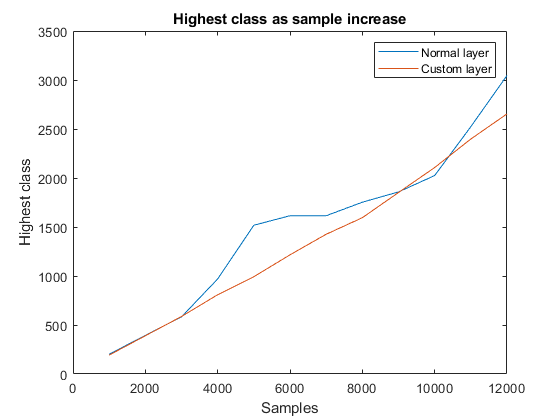
\includegraphics[width=\textwidth]{figures/firstmax.png}
        \caption{Highest class}
        \label{sfig:ex:extra:firstmax}
    \end{subfigure}
    \hfill
    \begin{subfigure}[b]{.45\textwidth}
        \centering
        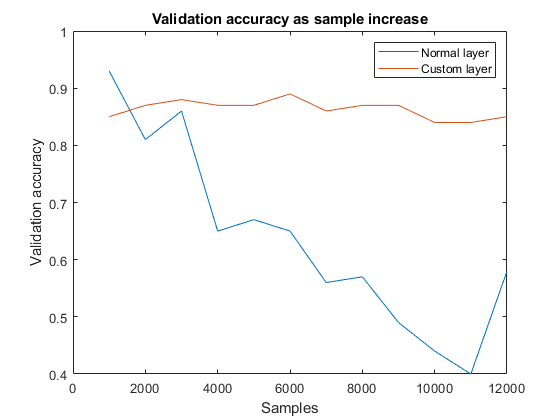
\includegraphics[width=\textwidth]{figures/firstres.png}
        \caption{Validation accuracy}
        \label{sfig:ex:extra:firstres}
    \end{subfigure}
    \caption{Largest class and validation accuracy as number of samples increase}
    \label{fig:ex:extra:firstresult}
\end{figure}

\begin{figure}
    \centering
    \begin{subfigure}[b]{.45\textwidth}
        \centering
        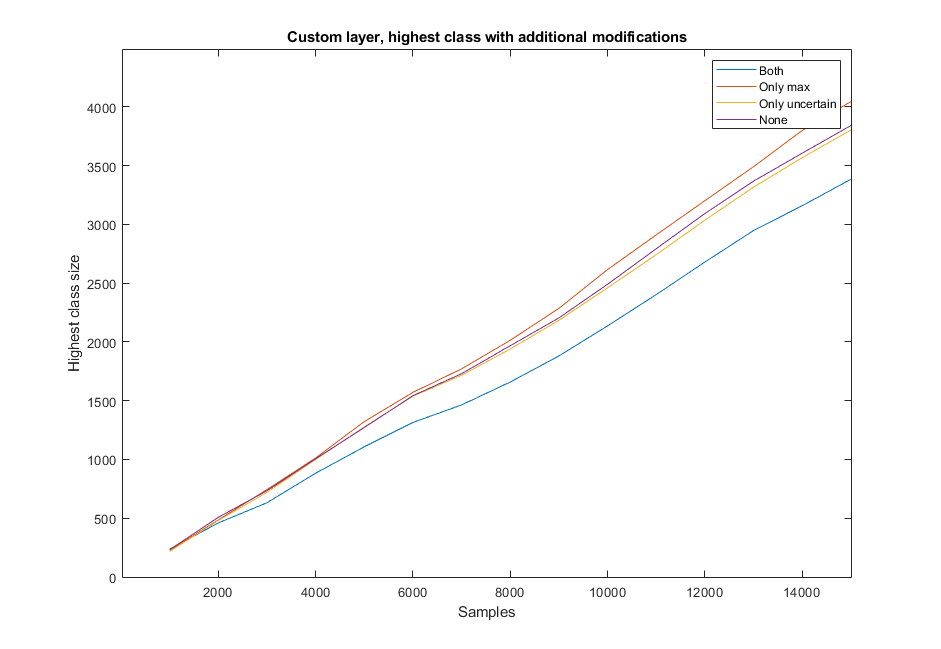
\includegraphics[width=\textwidth]{figures/customhigh.png}
        \caption{Custom layer largest class}
        \label{sfig:ex:extra:customhigh}
    \end{subfigure}
    \hfill
    \begin{subfigure}[b]{.45\textwidth}
        \centering
        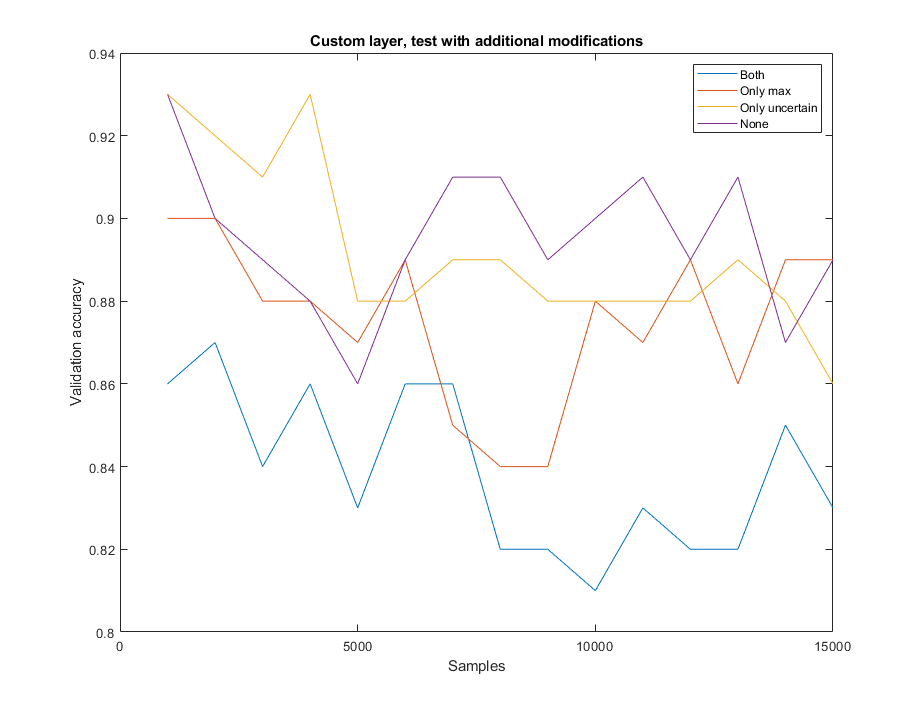
\includegraphics[width=\textwidth]{figures/customva.png}
        \caption{Custom layer val accuracy}
        \label{sfig:ex:extra:customva}
    \end{subfigure}
    \caption{Custom layer performance with the extra operations}
    \label{fig:ex:extra:custom}
\end{figure}

\begin{figure}
    \centering
    \begin{subfigure}[b]{.45\textwidth}
        \centering
        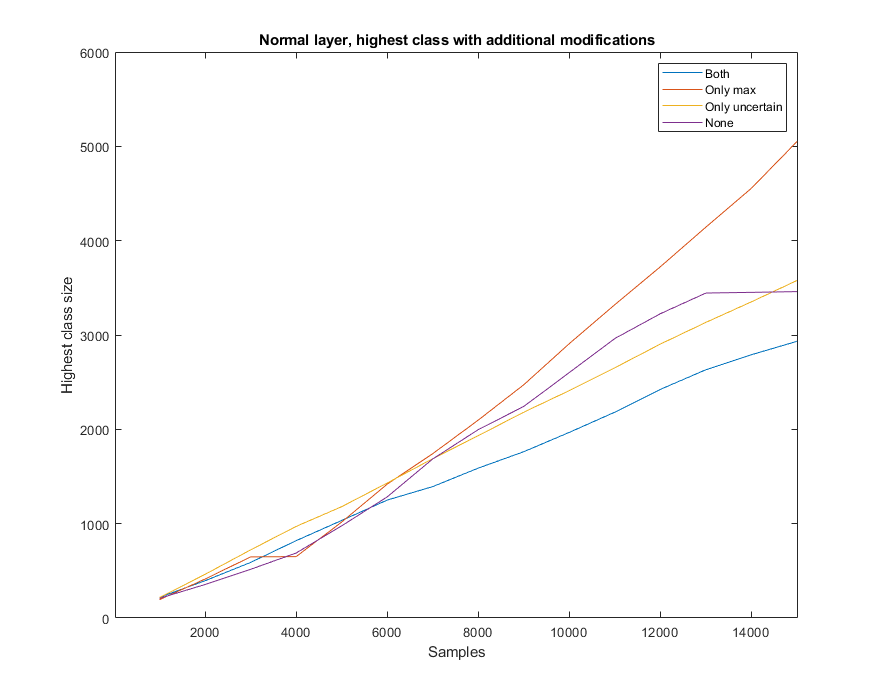
\includegraphics[width=\textwidth]{figures/normalhigh.png}
        \caption{Normal layer largest class}
        \label{sfig:ex:extra:normalhigh}
    \end{subfigure}
    \hfill
    \begin{subfigure}[b]{.45\textwidth}
        \centering
        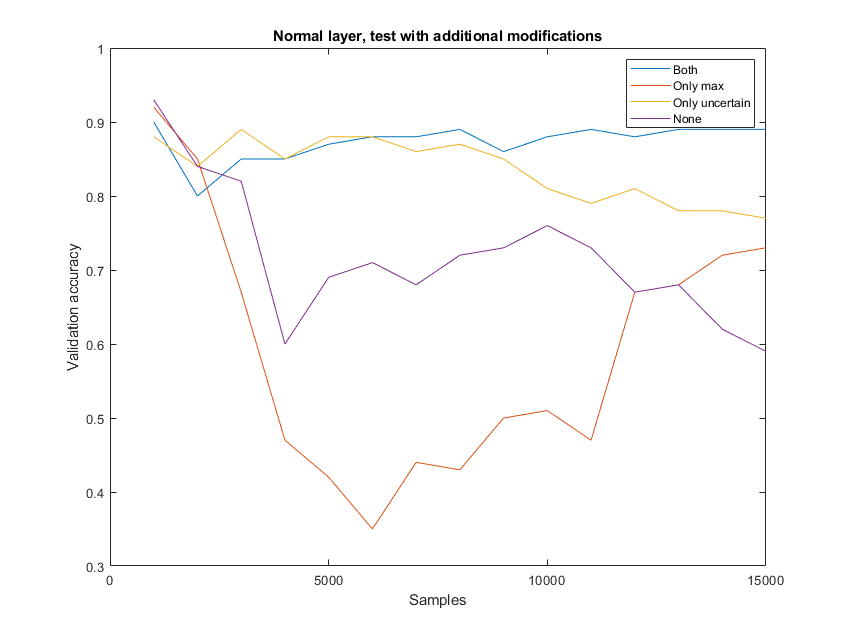
\includegraphics[width=\textwidth]{figures/normalva.png}
        \caption{Normal layer val accuracy}
        \label{sfig:ex:extra:normalva}
    \end{subfigure}
    \caption{Normal layer performance with the extra operations}
    \label{fig:ex:extra:normal}
\end{figure}


%Following the selection of the dataset, 1010 neuron idea was tested
%Custom layer was developed with the weights adjusted in the last 10 layers
%Pictures from APW report
%Additional theories tested, mention extra options, why they were not chosen (extra workload on processing, absolutely uninteresting results compared to just using custom layer and going forward)
%Important to mention as normal layer with both extra counter-measures appears to come close to custom layer results

\section{Neural network refinement experiments}
\label{ex:networkref}

During the refinement of the neural network model, the following workflow was adopted:

\begin{itemize}
    \item Determine the correct number of convolutional layers
    \item Test correct parameters to use in the conv layers
    \item Test the correct number of pooling layers, and their type
    \item Test the correct number of neurons in the first dense layer
\end{itemize}

The last three steps were repeated in combination or by themselves depending on the number of parameters tested.
Each of the tests generated thousands of results, of which most did not fall too far away from the best performing model.
Therefore, the feeling of urgency and strictness with the neural network model was not present during development.
Instead, this experiment aimed at being thorough in its trials, to make sure the experiment would not need to be repeated.

After many different combinations of neural network structures have been attempted, the structure of the model was finalized.
The final network structure can be seen in \cref{tab:finalmodel}.

\begin{table}[ht]
    \centering
    \begin{tabular}{|c|c|c|}
        \hline
        Layer type & Parameters & Activation\\ \hline
        Conv1d & 128 filters, size 2 & ReLU\\ \hline
        Max pool & Size 2 & ReLU\\ \hline
        Conv1d & 64 filters, size 3 & ReLU\\ \hline
        Average pool & Size 2 & ReLU\\ \hline
        Conv1d & 64 filters, size 4 & ReLU\\ \hline
        Max pool & Size 2 & ReLU\\ \hline
        Conv1d & 16 filters, size 4 & ReLU\\ \hline
        Average pool & Size 2 & ReLU\\ \hline
        Flatten & &\\ \hline
        Dense & 200 & ReLU\\ \hline
        Dense & 10 & Softmax \\ \hline
        Dense (custom) & 1010 & Sigmoid \\ \hline
    \end{tabular}
    \caption{Modified early neural network model}
    \label{tab:finalmodel}
\end{table}

%Section 3: Neural network development in spring
%Methodology writeup, tons of combinations
%Section 1 to find good number of conv layers
%Section 2 pre-3-cluster or layer freeze modelling, table with results and subsequent next tests
%Section 3 final model, based on later experience, model parameters did not appear to be all that relevant in the dataset


%Lots of graph pages in this section
%10-20 pages? but lots of pictures

\section{Loss function experiments}
\label{ex:loss}

A similar process has been adapted to what has been used in \cref{ex:networkref} to investigate the correct parameters to use to determine the loss function filter boundaries,
The parameters that were picked centered around the final output layer neurons divided by the number of classes that the samples could be allocated to.
Thus, the clusters that would be below average would be rewarded, while the massive clusters would be penalized.

In addition to these parameters, two other components were tested in this experiment.
The first component was the use of differently sized initial clusters generated by Scikit, to have a more generalized cluster in the beginning.
The second component aimed to freeze most of the layers of the network used in the loss function processing, to prevent the result from overfitting.
In the beginning, the model would only have its fresh final layer to train for a couple of epochs, until which point the softmax layer would also be opened for training, albeit at a reduced learning rate.
The goal of this layer freezing was to reduce the instability of the loss function processing, by making sure that the significant shifts in the clusters would need to be justified, rather than caused by a configuration error.

\subsection{Secondary filter}
\label{ex:loss:secondfilter}
During the early experimentation, the secondary filter described in \cref{me:secondfilter} has been tested with the rest of the parameters.
While the difference between the combinations not using the filter was negligible, it was on the negative side of the results.
As the secondary filter never added much to the results, only the removal of the first of the last neurons was kept.

\subsection{Correct cluster count reevaluation}
Following the first proper loss function experiment, it was revealed that all combinations of parameters have descended into three clusters.
After an investigation, it was discovered that the other clusters generated by Scikit were unlikely to ever generalize with the rest of the dataset, and thus would only pollute the results.
The loss function experiment has been rerun with only three clusters to correct for this error,

The code for the layers and the network was not adjusted to fit this discovery, as most of this code would remain dormant with no samples ever touching the extra nodes.
As the network was optimized with ten clusters in mind, one more optimization pass was run on the network to be sure that the model would be good.
Additionally, the parameters of the loss function experiment have been adjusted to fit the new three cluster output.

\subsection{Experiment results}

After the second loss function experiment has concluded, the following results were generated:

\begin{itemize}
    \item Filter 0: First parameter 200
    \item Filter 1: First parameter 200, second parameter 800
    \item Filter 2: First parameter 400
    \item Filter 3: First parameter 400, second parameter 850
    \item Best iteration cluster size: 2000 (2x1000)
    \item First epoch limit: 5
    \item Second epoch limit: 10 (total of 15)
\end{itemize}

%Section 4: Loss function hyperparams?
%Results justifying why I went with the loss function parameters, the final last result
%Q: Had a "bad" batch of results that maybe weren't as relevant, include but state it used an older version?



%Section 1 on before 3clusters
%Section 2 on before layer freeze attempt
%Section 3 final results, which were "best in class", some had more trouble while others didn't?

\section{Iterative re-training experiment}
\label{ex:iter-retrain}
%Section 5: Iterative training

\subsection{Parameters used}
\label{ex:iter-retrain:params}

The parameters used in the experiment are as follows:
\begin{itemize}
    \item Function option, -2, -1, 0, 1, 2, 3
    \item Iteration threshold: 0.5, 0.6, 0.7, 0.8, 0.9
\end{itemize}{}

The iteration threshold defines the limit of how low certainty a sample needs to have to become a part of the dataset.

The function options 0 to 3 refer to the results of the experiment in \cref{ex:loss}, and the \cref{fig:me:loss01} and \cref{fig:me:loss23} filters used in the custom loss function.
The option -1 is created to verify that the loss function filters are of any use.
Option -1 is defined not to have a custom loss function; instead, it uses the standard sparse categorical cross-entropy.
As the process of the re-classification also needs to be investigated, option -2 is created.
Option -2 uses the classifications found during the search for the bad samples as the actual classes to use in the classification.
Should the entire loss function process be compromised, while there is still some value to the iterative re-training itself, this option is expected to have the best results.

\subsection{Experiment process}
Most of the logical process behind the experiment can be found in \cref{me:iter-retrain}.

Among the practical decisions made during the experiment, was the resetting of the final classification layer and layer freezing during the model re-train, after the new classifications were acquired.
The process is similar to the one used in the loss function processing defined in \cref{ex:loss}; however, this process has three steps.
As the final classification layer carries the most dataset-specific conclusions about the previous iteration, this layer was removed and replaced with a fresh layer.
The final layer was then processed for a maximum of 20 epochs, with the remainder of the model frozen.
Following this training process, the second last layer is unfrozen, and the model is set to resume training with a reduced learning rate for another 20 epochs.
Once the training freezes again, all but the first four of the network layers are unfrozen, and the training continues for another five epochs.
An early stopping mechanism is used to prevent the model from needlessly churning the iterations, which stops the training process if the accuracy has not improved beyond 5\% in the last ten epochs.
Should this happen, the remaining epochs are transferred to the next training step to utilize.



\subsection{Experiment results}
The bulk of the results for this experiment can be found in \cref{res:iter}.
One variable parameter, however, had to be eliminated for the following tree experiment.
Based on the initial results of this experiment, it was discovered that in almost all cases, iteration threshold 0.6 and 0.7 fail to achieve functional three clusters.
As more and more observations were made on the results, it was determined that an iteration threshold of 0.8 would be used in the future experiment.

%Main section detailing the big results from iterative training, all different ways to arrange data
%Provide as broad of a platform for discussion in the next section
%As results are in next chapters, discuss experiment parameters and how the experiment went?
%More technical part compared to methodology

\section{Tree generation experiment}
\label{ex:tree}
%Section 6: Tree generation
\subsection{Parameters used}
\label{ex:treeparam}

The parameters used in this experiment are:

\begin{itemize}
    \item Function option, -3, -2, -1, 0, 1, 2, 3
    \item Cache threshold: 0.5, (0.2, 0.3, and 0.4 with -3 only)
\end{itemize}{}

The function options are mostly the same parameters as used in \cref{ex:iter-retrain:params}.
There is one new parameter called -3, which does not use any iterative re-training for the tree generation process.

The cache threshold option mimics the iterative threshold option, in that it determines if a sample is used for a purpose or not.
With this parameter, a classification value higher than the threshold is necessary for the sample to be inserted into the next branch layer in the tree.
The standard cache threshold value across most of the function options is 0.5.
As the tree generation is expected to last a while, option -3 has been used to generate other tree combinations that there was not enough time for the other function options.
Option -3 therefore uses cache thresholds 0.2, 0.3, and 0.4 in addition to 0.5.

Following the data from the previous experiment, an iteration threshold of 0.8 is used across the entire experiment.

\subsection{Experiment process}
At the start of the experiment, the networks generated in the previous experiment have been reused for this experiment.
As the results would have been the same, it served to cut down the time to start significantly.
A cache from the root node has been generated for each of the three clusters that would receive their own networks.

The process can be summarized as follows:
\begin{enumerate}
    \item Check if the node has at least 20'000 samples, delete node cache if not
    \item Create the initial cluster using Scikit - AgglomerativeClustering
    \item Train the first network iteration
    \item Use iterative training (except -3) to create a new neural network
    \item Create cache for the next branch layer
    \item Repeat until no more cache folders to process
\end{enumerate}

In addition to creating the cache for the next branch layer, should a node cluster so severely that it put all of its samples into the same cluster, that cluster is removed.
These steps have utilized all available hard disk drives as caches for the tree generation, as each of the options had to have its copy of the dataset, in the case of the control options, even more than one copy.



%Same but for trees
%Uses resulting networks from iter train as root nodes, since it's same shit
%Based on the cluster collapse down to 2 clusters in previous experiment, uses 0.8 as threshold for training
%0.5 as default threshold to be used in next tree, control version -3 could afford smaller numbers
%Time it takes to generate trees, mention how combination 3 finished on FUCKING FRIDAY before report handin?
%As many results as possible for the discussion section
\subsection{Experiment results}
All of the results for this experiment can be found in \cref{res:tree}.